\documentclass[
    % fontset=ubuntu, % 生僻字可用思源字体,如“昇腾”
    fontset=fandol,
    xcolor=svgnames % SeaGreen
]{ctexbeamer}

\usetheme[
    compress % 进度条压缩在一行,可选
]{Berlin}

\usecolortheme[named=SeaGreen]{structure}

\title{OSM: Off-Chip Shared Memory for GPUs}

\subtitle{分享:吴坎}

\author[Sina Darabi et al.]{Sina Darabi, Ehsan Yousefzadeh-Asl-Miandoab, Negar Akbarzadeh, Hajar Falahati, Pejman Lotfi-Kamran, Mohammad Sadrosadati, Hamid Sarbazi-Azad}

\institute[Sharif University of Technology / ETH Zürich]{
    
\includegraphics[height=0.07\textheight]{assets/logo/logo0409.png}
}

\logo{
\includegraphics[height=0.07\textheight]{assets/logo/arcsysu.png}}

\date{
    %\today
    二〇二二年十月
}

\begin{document}

\section{Introduction}

\subsection{Weekly Paper Sharing}

\begin{frame}

    \titlepage

\end{frame}

\begin{frame}

    \begin{block}{About this paper}
        \begin{itemize}
            \item \href{https://ieeexplore.ieee.org/xpl/RecentIssue.jsp?punumber=71}{Published in: IEEE Transactions on Parallel and Distributed Systems} ( Volume: 33, \href{https://ieeexplore.ieee.org/xpl/tocresult.jsp?isnumber=9790018&punumber=71}{Issue: 12}, 01 December 2022)
            \item DOI: \href{https://doi.org/10.1109/TPDS.2022.3154315}{10.1109/TPDS.2022.3154315}
        \end{itemize}
    \end{block}

    \begin{block}{Another noteworthy paper}
        \begin{itemize}
            \item Sina Darabi, Mohammad Sadrosadati, Joël Lindegger, Negar Akbarzadeh, Mohammad Hosseini, Jisung Park, Juan Gómez-Luna, Hamid Sarbazi-Azad, Onur Mutlu. Morpheus: Extending the Last Level Cache Capacity in GPU Systems Using Idle GPU Core Resources. MICRO 2022.
            \item DOI: \href{https://doi.org/10.48550/arXiv.2209.10914}{10.48550/arXiv.2209.10914}
        \end{itemize}
    \end{block}

\end{frame}

\subsection{Motivation}

\begin{frame}

    \begin{block}{Shared memory: software-managed cache in each SM of GPU}
        \begin{itemize}
            \item accelerate data sharing across threads of a thread block
            \item save significant amount of GPU
                  power
        \end{itemize}
    \end{block}

    \begin{block}{However\dots}
        \begin{itemize}
            \item most of the workloads
                  do not fully utilize the allocated shared memory space
            \item limit the number of allocated thread blocks in each SM, and potentially thread-level parallelism (TLP)
        \end{itemize}
    \end{block}

\end{frame}

\begin{frame}

    \begin{figure}
        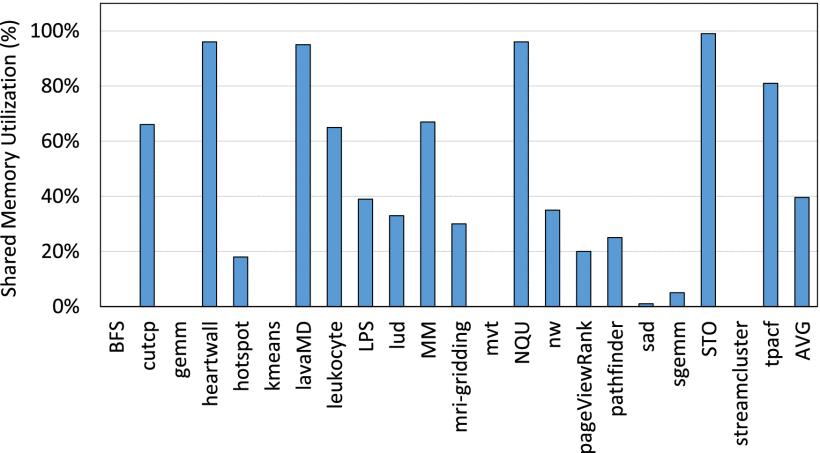
\includegraphics[width=1\textwidth]{assets/figure/sadro1-3154315-large.png}
        \caption{Shared memory utilization across 22 workloads; 5 workloads out of 22 do not utilize shared memory at all.}
    \end{figure}

\end{frame}

\begin{frame}

    \begin{block}{Main bottleneck of shared memory}
        \begin{itemize}
            \item will not be freed till
                  the end of the thread block execution
            \item lifetime range of smem is about $50\times$ shorter than the thread block execution time on average
        \end{itemize}
    \end{block}

    \begin{figure}
        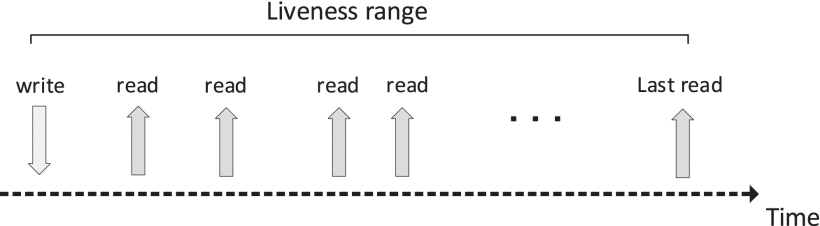
\includegraphics[width=1\textwidth]{assets/figure/sadro2-3154315-large.png}
        \caption{lifetime range of a shared memory address.}
    \end{figure}

\end{frame}

\begin{frame}

    \begin{figure}
        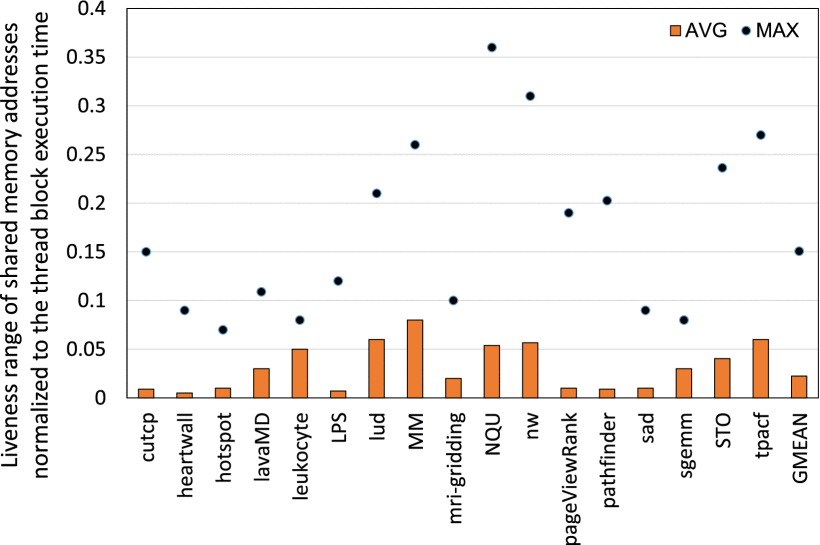
\includegraphics[height=0.8\textheight]{assets/figure/sadro3-3154315-large.png}
        \caption{Average and maximum lifetime range of shared memory addresses for the workloads that utilize shared memory.}
    \end{figure}

\end{frame}

\begin{frame}
    \begin{block}{So\dots}
        \begin{itemize}
            \item need to modify the cache management
            \item do not need to keep these addresses for the entire execution time of a thread block
        \end{itemize}
    \end{block}
\end{frame}

\subsection{Background}

\begin{frame}

    \begin{block}{GPU Architecture}
        \begin{itemize}
            \item SM,CTA,warp,rigister file,load/store units,bank conflicts\dots
        \end{itemize}
    \end{block}

    \begin{block}{GPU Memory System}
        \begin{itemize}
            \item on-chip: Unified shared memory/texure memory L1,L2
            \item off-chip: device memory
        \end{itemize}
    \end{block}

    \begin{figure}
        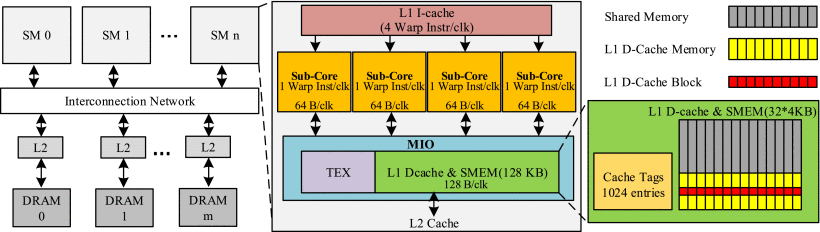
\includegraphics[width=1\textwidth]{assets/figure/sadro4-3154315-large.png}
        \caption{GPU architecture.}
    \end{figure}

\end{frame}

\section{Off-Chip Shared Memory (OSM)}

\begin{frame}

    \begin{block}{Design}
        \begin{itemize}
            \item allocates shared memory address space in the off-chip memory
            \item accelerates its accesses using an on-chip shared memory cache
            \item add a bit to each cache block tag for lock/unlock mechanism
        \end{itemize}
    \end{block}

    \begin{figure}
        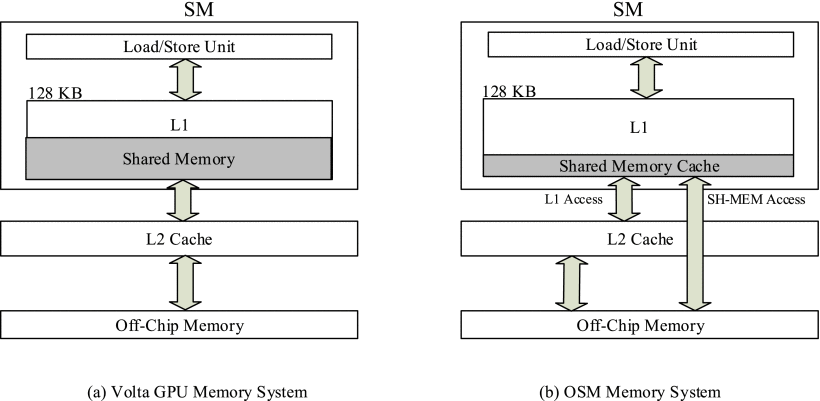
\includegraphics[height=0.5\textheight]{assets/figure/sadro5-3154315-large.png}
        \caption{Baseline GPU memory system vs. OSM memory system.}
    \end{figure}

\end{frame}

\begin{frame}

    \begin{block}{Write-back
            policy for the added shared memory cache}
        \begin{itemize}
            \item shared memory addresses are shared only across threads in a thread block of an SM
            \item only write data in the cache at the request time
            \item written back to the shared memory space of off-chip memory on its eviction at some later time
        \end{itemize}
    \end{block}

    \begin{block}{keep in the cache during its lifetime range}
        \begin{itemize}
            \item run-time measurement of lifetime ranges is impractical
            \item predict the lifetime ranges through studying the write/read pattern of shared memory addresses
        \end{itemize}
    \end{block}
\end{frame}

\begin{frame}

    \begin{figure}
        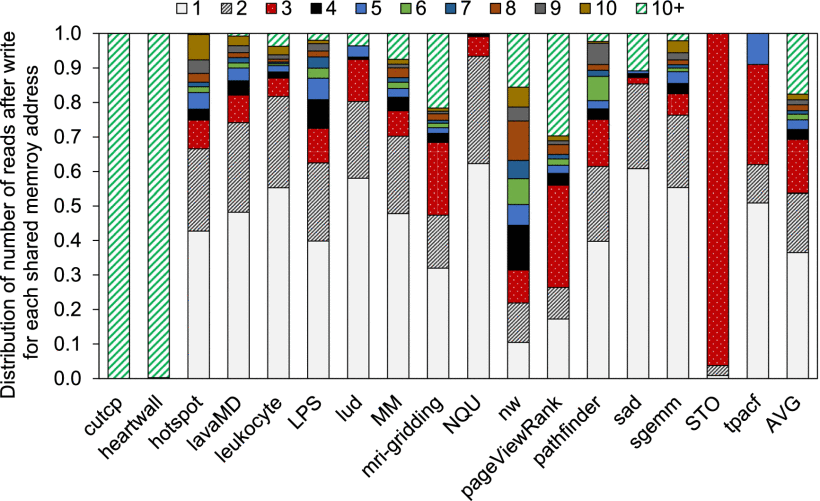
\includegraphics[width=1\textwidth]{assets/figure/sadro6-3154315-large.png}
        \caption{Distribution of read accesses during their lifetime range for the workloads that utilize the shared memory during the execution.}
    \end{figure}

\end{frame}

\begin{frame}

    \begin{block}{lock/unlock mechanism}
        \begin{itemize}
            \item lock a shared memory address in the cache when it is written
            \item unlock it after a certain number of reads
            \item statically set this threshold to one
            \item those have frequent reads during their lifetime are likely kept in the cache based on the LRU replacement policy
        \end{itemize}
    \end{block}

\end{frame}

\begin{frame}

    \begin{block}{moves the shared memory address space to off-chip memory}
        \begin{itemize}
            \item a larger space than the limited on-chip SRAM space
            \item improve the thread-level parallelism (TLP)
            \item accordingly the performance of the workloads whose number of thread blocks is limited by the insufficient on-chip shared memory space
        \end{itemize}
    \end{block}

\end{frame}

\begin{frame}

    \begin{block}{UCM: unified cache memory}
        \begin{itemize}
            \item improve design by unifying the SMEM cache and L1-D cache
            \item bypass the L2 cache for accesses to the OSM
        \end{itemize}
    \end{block}

    \begin{figure}
        \begin{minipage}{0.49\textwidth}
            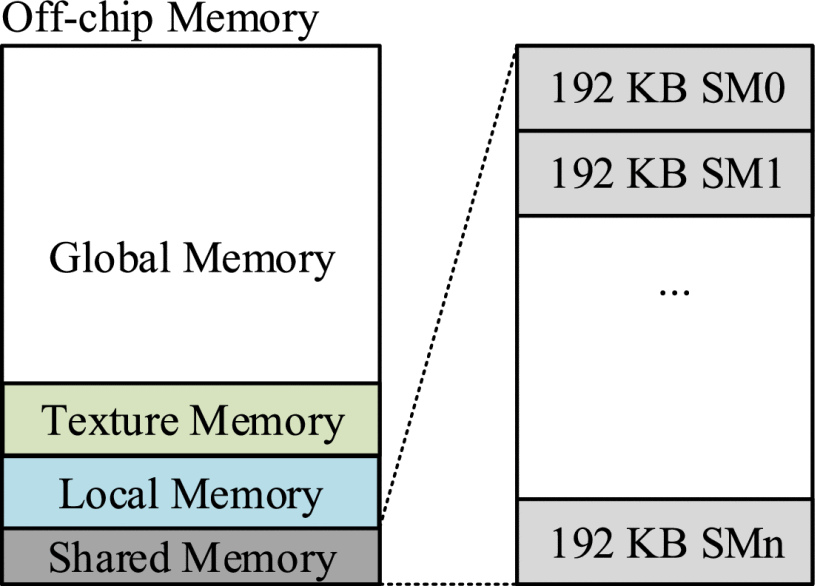
\includegraphics[height=0.45\textheight]{assets/figure/sadro7-3154315-large.png}
            \caption{Unified addressing map to off-chip memory (a.k.a., device memory).}
        \end{minipage}
        \begin{minipage}{0.49\textwidth}
            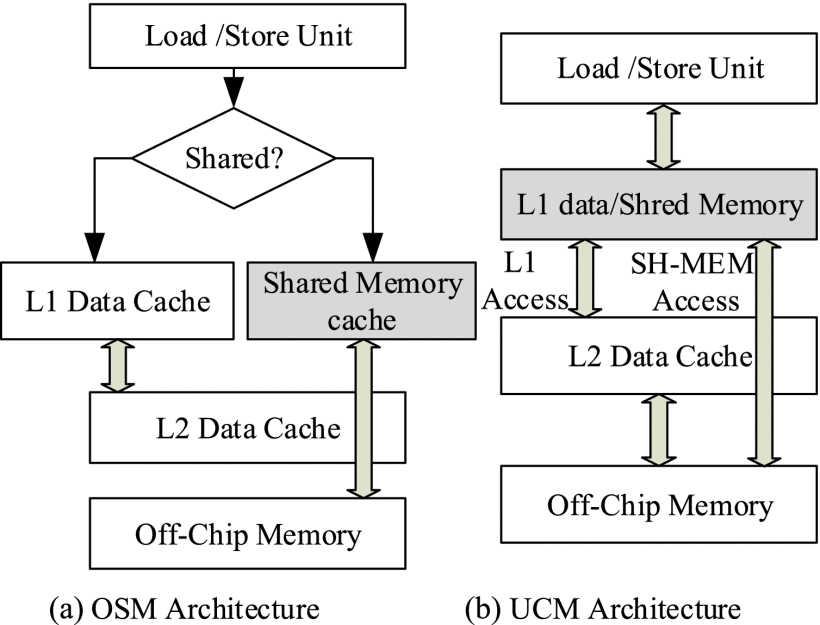
\includegraphics[height=0.45\textheight]{assets/figure/sadro8-3154315-large.png}
            \caption{Unified L1 data cache and shared memory cache.}
        \end{minipage}
    \end{figure}

\end{frame}

\begin{frame}

    \begin{figure}
        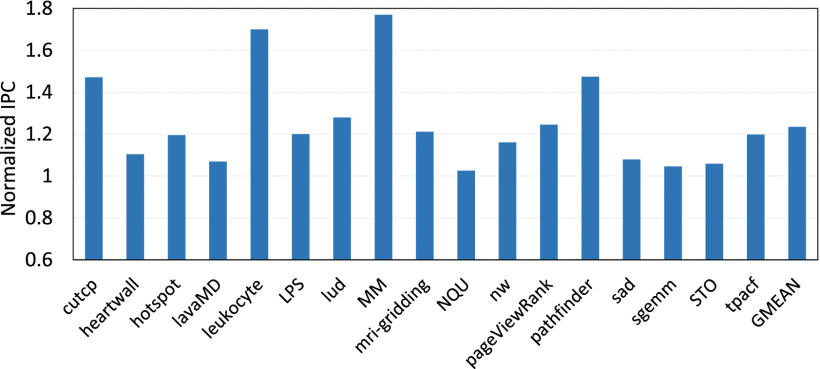
\includegraphics[width=1\textwidth]{assets/figure/sadro9-3154315-large.png}
        \caption{Performance improvement of an idealized GPU with 96 KB shared memory and 128 KB L1 data cache compared to the baseline Volta architecture for the workloads that utilize the shared memory.}
    \end{figure}

\end{frame}

\section{Methodology}

\begin{frame}
    \begin{block}{Simulation}
        \begin{itemize}
            \item Use Accel-Sim  and GPU-Wattch with a Volta-like configuration
        \end{itemize}
    \end{block}

    \begin{block}{Benchmark}
        \begin{itemize}
            \item 22 workloads from CUDA SDK, Rodinia, Parboil, Mars, and PolyBench
            \item categorize workloads in 3 groups including:
                  \begin{enumerate}
                      \item shared memory is not used
                      \item shared memory is used (TLP is not limited)
                      \item shared memory is used (TLP is limited)
                  \end{enumerate}
        \end{itemize}
    \end{block}
\end{frame}

\begin{frame}

    \begin{block}{Comparison Points}
        \begin{itemize}
            \item vary the size of shared memory cache to find the optimal point at which the performance remains unchanged
                  \begin{enumerate}
                      \item the baseline GPU architecture
                      \item OSM without lock/unlock mechanism (OSM-no-lock)
                      \item OSM
                  \end{enumerate}
            \item the effectiveness of the UCM proposal         \begin{enumerate}
                      \item Baseline NVIDIA Volta architecture
                      \item Unified on-chip memories proposed by Gebhart et al.\footnote{M. Gebhart, S. W. Keckler, B. Khailany, R. Krashinsky and W. J. Dally, "Unifying primary cache scratch and register file memories in a throughput processor", Proc. 45th Annu. IEEE/ACM Int. Symp. Microarchit., pp. 96-106, 2012.}
                      \item UCM
                  \end{enumerate}
        \end{itemize}
    \end{block}

\end{frame}

\section{Evaluation}

\subsection{OSM Analysis}

\begin{frame}

    \begin{figure}
        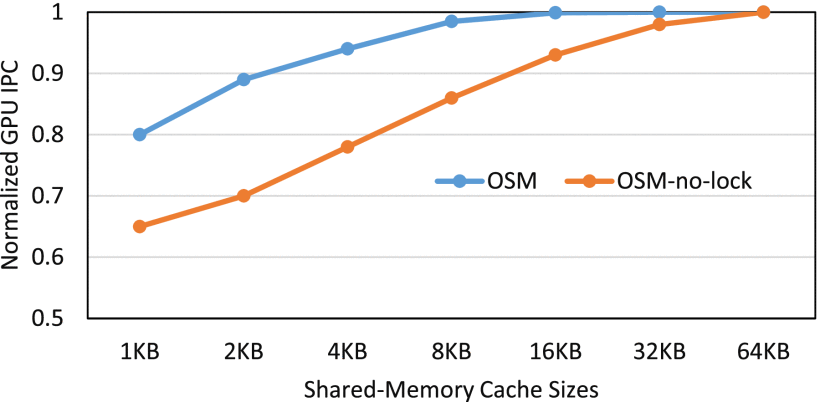
\includegraphics[width=1\textwidth]{assets/figure/sadro10-3154315-large.png}
        \caption{GPU performance using OSM and OSM-no-lock.}
    \end{figure}

\end{frame}

\begin{frame}

    \begin{figure}
        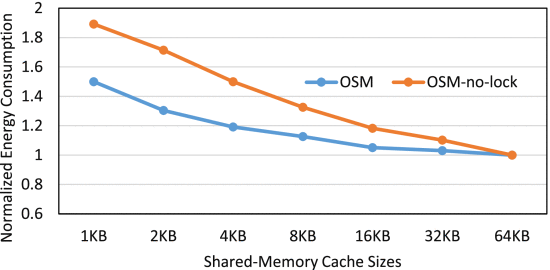
\includegraphics[width=1\textwidth]{assets/figure/sadro11-3154315-large.png}
        \caption{Energy consumption using OSM and OSM-no-lock.}
    \end{figure}

\end{frame}

\begin{frame}

    \begin{figure}
        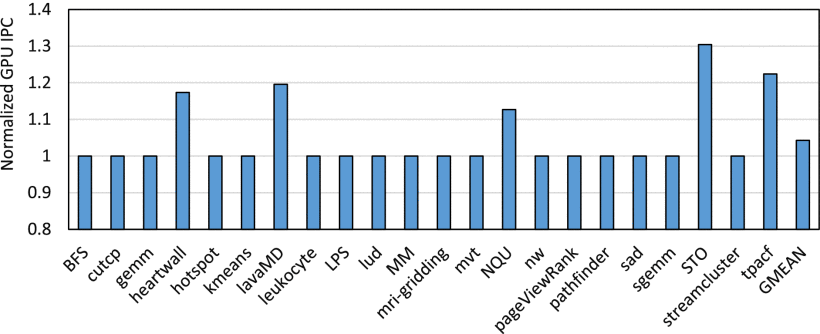
\includegraphics[width=1\textwidth]{assets/figure/sadro12-3154315-large.png}
        \caption{GPU IPC of 2× larger shared memory using OSM.}
    \end{figure}

\end{frame}

\begin{frame}

    \begin{block}{Two Key Observations}
        \begin{itemize}
            \item OSM provides almost the same performance with a reasonable energy overhead using small (8KB) cache sizes
            \item the lock/unlock mechanism is effective in increasing the performance and decreasing the consumed power
        \end{itemize}
    \end{block}

    \begin{block}{Effectiveness of OSM}
        \begin{itemize}
            \item increasing logical shared memory space, realized in the off-chip memory, to remove the TLP limitation
            \item caching SMEM space on-chip to hide the long off-chip memory access latency
            \item devising a lock/unlock mechanism to address lifetime issue
        \end{itemize}
    \end{block}

\end{frame}

\subsection{Overall Effect on GPU Performance}

\begin{frame}

    \begin{figure}
        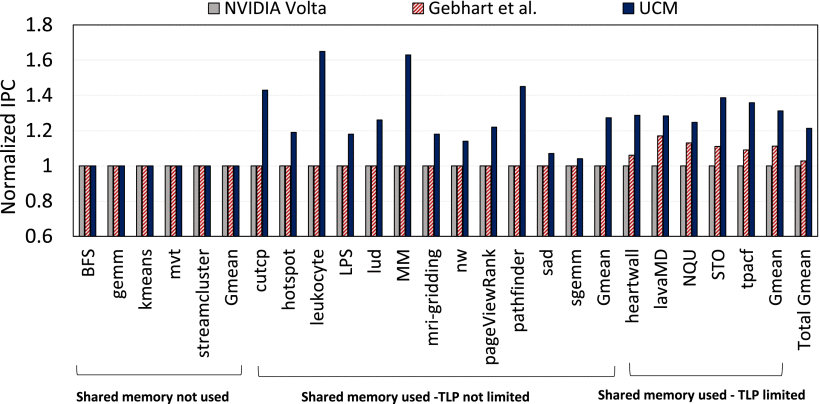
\includegraphics[width=1\textwidth]{assets/figure/sadro13-3154315-large.png}
        \caption{GPU overall IPC results normalized to the baseline Volta architecture.}
    \end{figure}

\end{frame}

\subsection{Overall Effect on GPU Energy Consumption}

\begin{frame}

    \begin{figure}
        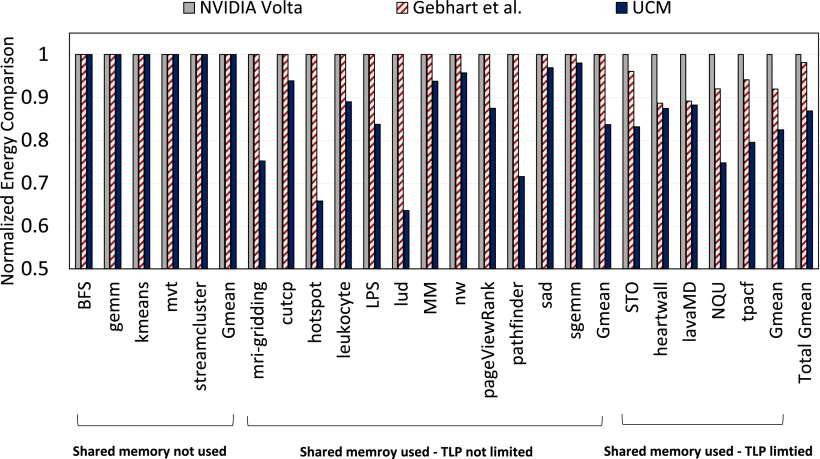
\includegraphics[width=1\textwidth]{assets/figure/sadro14-3154315-large.png}
        \caption{Energy consumption comparison..}
    \end{figure}

\end{frame}

\subsection{Analysis of Reads-to-Unlock Threshold}

\begin{frame}

    \begin{block}{The sensitivity of the proposal to the threshold}
        \begin{itemize}
            \item Ideal: dynamically changes the threshold of each address
            \item Utilizing a complex technique for the ideal case is not worthy
        \end{itemize}
    \end{block}

    \begin{figure}
        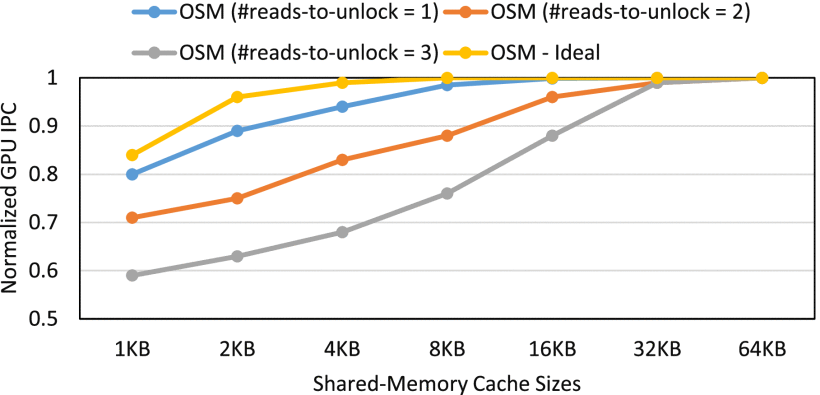
\includegraphics[width=0.8\textwidth]{assets/figure/sadro15-3154315-large.png}
        \caption{Impact of read to unlock threshold on performance improvement.}
    \end{figure}

\end{frame}

\subsection{Accuracy of Shared Memory Cache Eviction Policy}

\begin{frame}

    \begin{figure}
        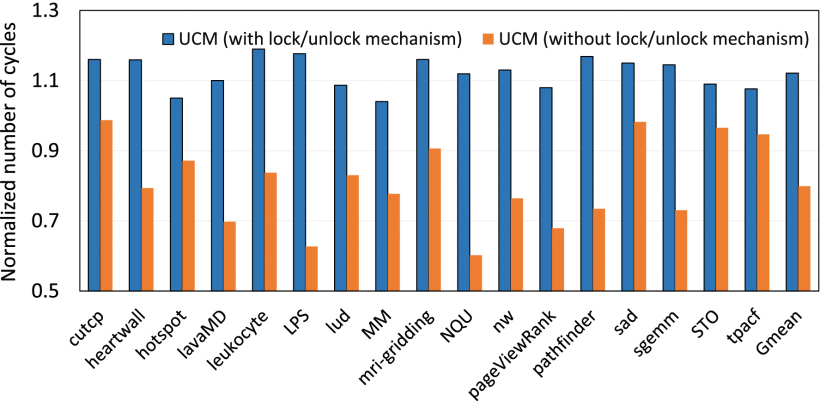
\includegraphics[width=1\textwidth]{assets/figure/sadro16-3154315-large.png}
        \caption{Effect of lock/unlock mechanism on keeping shared memory addresses in the cache during their lifetime range.}
    \end{figure}

\end{frame}

\begin{frame}

    \begin{block}{without lock/unlock mechanism}
        \begin{itemize}
            \item addresses of shared memory are evicted too early
            \item need to be returned to the cache again
            \item can cause performance and energy overheads
        \end{itemize}
    \end{block}

    \begin{block}{with lock/unlock mechanism}
        \begin{itemize}
            \item each shared memory address is evicted a bit late
            \item it cannot be evicted after unlocking unless the LRU policy chooses it as a victim block
        \end{itemize}
    \end{block}

\end{frame}

\subsection{Sensitivity on GPU Bandwidth}

\begin{frame}

    \begin{figure}
        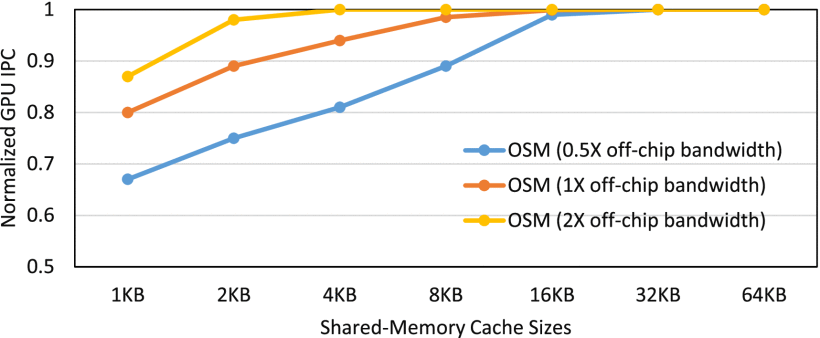
\includegraphics[width=1\textwidth]{assets/figure/sadro17-3154315-large.png}
        \caption{Off-chip memory bandwidth sensitivity analysis.}
    \end{figure}

\end{frame}

\begin{frame}

    \begin{figure}
        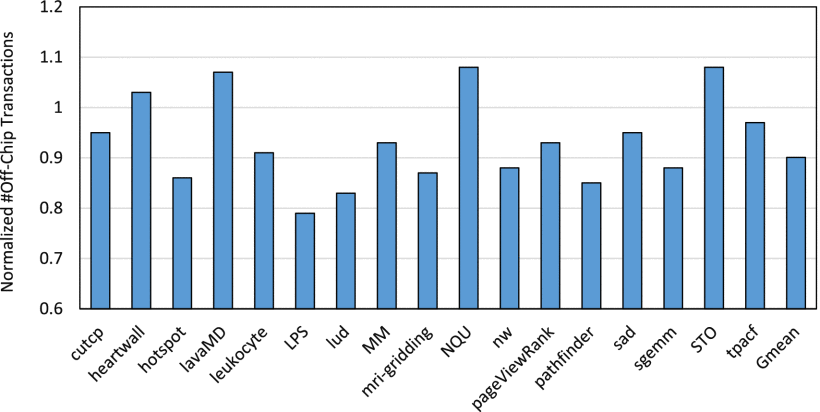
\includegraphics[width=1\textwidth]{assets/figure/sadro18-3154315-large.png}
        \caption{Off chip transaction of workloads that utilize shared memory.}
    \end{figure}

\end{frame}

\section{Conclusion}

\begin{frame}

    \begin{block}{the utilization and lifetime of shared memory addresses in GPUs}
        \begin{itemize}
            \item shared memory is not well-utilized \item its lifetime is much shorter than the thread block execution
        \end{itemize}
    \end{block}

    \begin{block}{keep SMEM in off-chip memory and accelerate via on-chip cache}
        \begin{itemize}
            \item improves the TLP for the workloads which TLP is limited by shared memory
            \item increases the on-chip cache memory capacity and bandwidth
            \item an average 21\% IPC improvement compared to the baseline
        \end{itemize}
    \end{block}

\end{frame}

\subsection{Q \& A}

\begin{frame}

    \begin{block}{Questions?}
        ~\\
        ~\\
        \center{\Large{Thank you!}}\\
        ~\\
        ~\\
        ~\\
        ~\\
    \end{block}

\end{frame}

\end{document}